\documentclass[10pt,pdf,hyperref={unicode}]{beamer}

\usepackage[utf8]{inputenc}
\usepackage[english,russian]{babel}
\usepackage{amsmath,amssymb}
\usefonttheme[onlymath]{serif}
\setbeamercovered{transparent}
\usepackage{amsthm}
\usepackage{color}
\usepackage{tikz}
\usepackage{graphicx}
\usepackage{caption}
\usepackage{subcaption}
\usepackage{epstopdf}
\usepackage{listings}
\lstdefinestyle{mycode}{
  belowcaptionskip=1\baselineskip,
  breaklines=true,
  xleftmargin=\parindent,
  showstringspaces=false,
  basicstyle=\footnotesize\ttfamily,
  keywordstyle=\bfseries,
  commentstyle=\itshape\color{red},
  stringstyle=\color{red},
  numbers=left,
  numbersep=5pt,
  numberstyle=\tiny\color{gray},
}
\lstset{style=mycode}

\hyphenpenalty=10000

\title{Разработка системы для статического контроля изменяемости объектов в объектно-ориентированных языках на основе JVM}

\usetheme{Boadilla}

\author[А. Д. Ждан]{Магистрант:~Анна~Ждан ~~~~~~Научный~руководитель:~А. А. Бреслав~~~~~~}
\institute[СПбАУ НОЦНТ РАН]{Учреждение Российской академии наук Санкт-Петербургский Академический университет — научно-образовательный центр нанотехнологий РАН}

\makeatletter
\defbeamertemplate*{footline}{my theme}{
    \leavevmode%
    \hbox{%
    \begin{beamercolorbox}[wd=.55\paperwidth,ht=2.25ex,dp=1ex,center]{author in head/foot}%
        \usebeamerfont{author in head/foot}%
        \insertshortauthor~~\beamer@ifempty{\insertshortinstitute}{}{(\insertshortinstitute)}
    \end{beamercolorbox}%
%    \begin{beamercolorbox}[wd=.43\paperwidth,ht=2.25ex,dp=1ex,center]{title in head/foot}%
%        \usebeamerfont{title in head/foot}\inserttitle
%    \end{beamercolorbox}%
    \begin{beamercolorbox}[wd=.45\paperwidth,ht=2.25ex,dp=1ex, center]{date in head/foot}%
        \usebeamerfont{date in head/foot}\insertshortdate{}\hspace*{1em}
        \insertframenumber{} / \inserttotalframenumber
    \end{beamercolorbox}}%
}
\makeatother



\begin{document}
\begin{frame}[plain]
\maketitle
\end{frame}


\begin{frame}
	\transwipe
	\frametitle{Предметная область}
\begin{center}
Неизменяемый объект~~~~~~~~Неизменяемая ссылка
\end{center}
\begin{figure}[h]
\centering
	\begin{subfigure}[b]{0.45\textwidth}
		\raggedleft
    	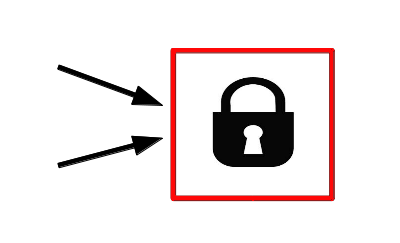
\includegraphics[scale=0.25]{pics/2.png}
	\end{subfigure}
	\begin{subfigure}[b]{0.45\textwidth}
		\raggedright
    	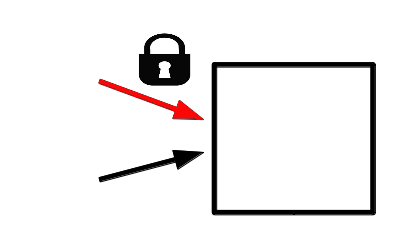
\includegraphics[scale=0.25]{pics/4.png}
	\end{subfigure}
\end{figure}
\begin{figure}[p]
	\begin{subfigure}[b]{0.6\textwidth}
		\centering
		Глубокая неизменяемость
    	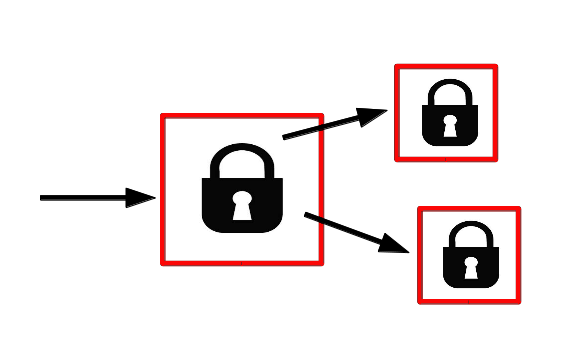
\includegraphics[scale=0.25]{pics/3.png}
	\end{subfigure}	
\end{figure}
\end{frame}



%\begin{frame}
%	\transwipe
%	\frametitle{Выявление ошибок на этапе компиляции}
%	
%	\begin{itemize}	
%	\item
%		ошибки при нарушении инкапсуляции	
%	\item
%		ошибки при параллельном программировании
%	\end{itemize}
	
%\end{frame}
\begin{frame}
	\transwipe
	\frametitle{Цели и задачи работы}
	Цель работы:
	\begin{itemize}
	\item
	Контролировать изменяемость объектов на этапе компиляции
	\end{itemize}

	Задачи:
	\begin{itemize}
	\item 
		формальная система аннотаций,
	\item 
		автоматический вывод аннотаций.
	\end{itemize}
\end{frame}

\begin{frame}[fragile]
	\transwipe
	\frametitle{Существующие решения}
\begin{center}
	\begin{tabular}{ | p{3.5cm} | p{0.9cm} | p{0.9cm} | p{0.9cm} | p{0.9cm} | p{0.9cm} |}
	\hline  & C++ & Java & Javari & IGJ & Gordon 2012 \\
	\hline глубокая неизменяемость & +/- & - & + & + & + \\
	\hline полиморфизм & - & - & + & + & + \\
	\hline объектная неизменяемость & + & + & - & + & + \\
	\hline ссылочная неизменяемость & - & - & + & + & + \\
	\hline циклы неизменяемых объектов & - & - & - & - & + \\
	\hline автоматическое аннотирование библиотек & N/A & N/A & + & - & - \\
	\hline
    \end{tabular}
\end{center}
	
\end{frame}



\begin{frame}
	\transwipe
	\frametitle{Предлагаемая система аннотаций}
	\begin{columns}[t] 
    \column{.5\textwidth} % column designated by a command
     Аннотации на переменных, параметрах метода, возвращаемых значениях: 
	\begin{itemize}
	\item @ReadOnly 
	\item @Immutable 
	\item @Mutable
	\item @Isolated 
	\item @AsClass
	\end{itemize}
    \column{.1\textwidth}
    \column{.4\textwidth}
     Аннотации на методах:
	\begin{itemize}
	\item @Const
	\item @Pure
	\end{itemize}
	Аннотации на полях: 
	\begin{itemize}
	\item @Transient
	\item @ReadOnly
	\item @Immutable
	\item @Mutable
	\item @AsClass
	\end{itemize} 
    \end{columns}
\end{frame}

\lstset{language=java}
\begin{frame}[fragile]
	\transwipe
	\frametitle{Пример использования аннотаций}
\begin{lstlisting}
public class Person {
    @AsClass private Date dateOfBirth;
		
    @Const
    @ReadOnly 
    public Date getDateOfBirth() {return dateOfBirth;}

    public void setDateOfBirth(@AsClass Date dateOfBirth) {
        this.dateOfBirth = dateOfBirth;
    }
}
	...
    @Immutable Person p1 = new Person();		
    p1.getDateOfBirth();
    p1.setDateOfBirth(...); //compilation error
	
	\end{lstlisting}
\end{frame}

\lstset{language=java}
\begin{frame}[fragile]
	\transwipe
	\frametitle{Вывод аннотаций}
	
	\begin{lstlisting}
public class MyClass {
	
    @[Method mutability]
    @[Method purity]
    @[Return value mutability]
    public MyClass doSmth(@[?] Date p1, @[?] Date p2) {...}

    @[Return value mutability]
    public static Date foo(@[?] Date p1) {...}
							  
}	
	\end{lstlisting}
\end{frame}



\begin{frame}
	\transwipe
	\frametitle{Вывод аннотаций}
	\begin{figure}[p]
		\centering
		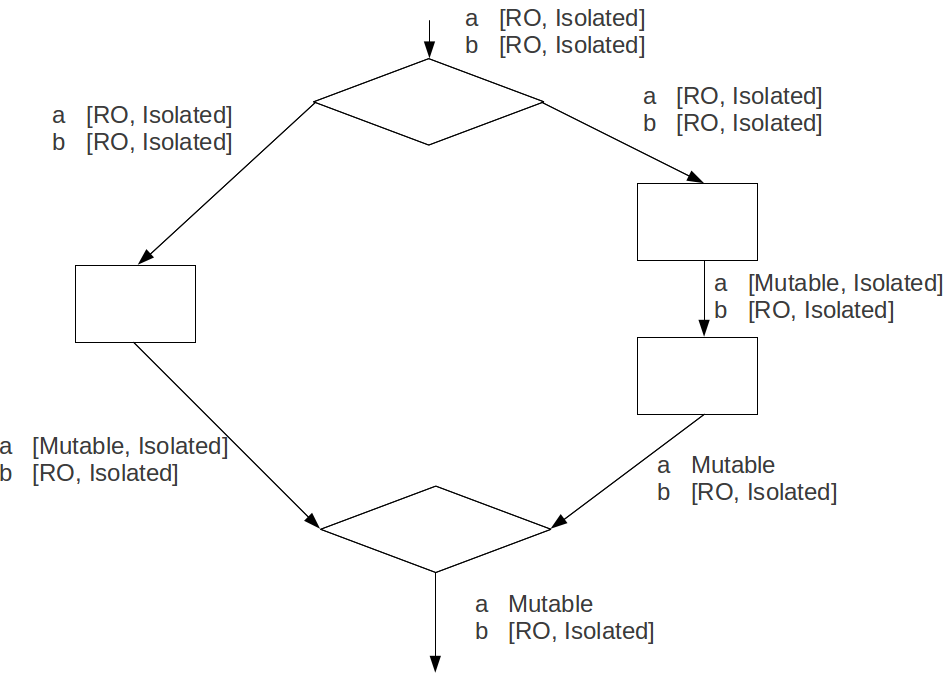
\includegraphics[scale=0.25]{pics/1.png}
\end{figure}
\end{frame}



\begin{frame}[fragile]
	\transwipe
	\frametitle{Сравнение с существующими решениями}
\begin{center}
	\begin{tabular}{ | p{3.5cm} | p{0.9cm} | p{0.9cm} | p{0.9cm} | p{0.9cm} | p{0.9cm} | p{1.1cm} |}
	\hline  & C++ & Java & Javari & IGJ & Gordon 2012 & \textbf{эта работа} \\
	\hline глубокая неизменяемость & +/- & - & + & + & + & \textbf{+} \\
	\hline полиморфизм & - & - & + & + & + & \textbf{+} \\
	\hline объектная неизменяемость & + & + & - & + & + & \textbf{+} \\	
	\hline ссылочная неизменяемость & - & - & + & + & + & \textbf{+} \\
	\hline циклы неизменяемых объектов & - & - & - & - & + & \textbf{+} \\
	\hline автоматическое аннотирование библиотек & N/A & N/A & + & - & - & \textbf{+} \\
	\hline
    \end{tabular}
\end{center}
\end{frame}




\begin{frame}
	\transwipe
	\frametitle{Результаты}
	\begin{itemize}
	\item
	Разработана система аннотаций, позволяющая выражать объектную и ссылочную неизменяемость.
	\item
	Разработан алгоритм, позволяющий вывести аннотации для существующего байт-кода.	
	\end{itemize}
\end{frame}




\begin{frame}
	\transwipe
\centering
{\huge Спасибо за внимание!}

\end{frame}


\end{document}
































